\documentclass[UTF8]{ctexart}

% 参考文献
\bibliographystyle{plain} % 声明参考文献格式
\usepackage{url}


% 设置页边距
\usepackage{geometry}
\geometry{a4paper,scale=0.8}

% 插入PDF
\usepackage{pdfpages}

% 插图功能的相关宏包
\usepackage{graphicx}
\usepackage{float}
\graphicspath{{figures/}}

% % 修改字体
% \usepackage{type1cm}  %(其中的 cm 为 Computer Modern 的缩写)
% \CJKfamily{song}  % 宋体

% 增加目录中的项目用tocbibind
\usepackage[nottoc]{tocbibind}
% 宏会默认增加目录本身,参考文献,索引等项目.noctoc取消了目录中显示目录
\begin{document}


\includepdf[pages={1}]{cover.pdf}
\newpage
\tableofcontents

\section{问题描述}
  设计一个程序实现对宾馆房间的基本管理,可以实现:
  \begin{itemize}
    \item 客房信息的录入功能;
    \item 客人入住登记
    \item 客人退房结算
    \item 客房信息浏览功能
    \item 浏览全部客户的信息,
    \item 客房信息和客户信息分别保存于不同文件;
    \item 客房信息查询,
    \item 查询空房间情况,
    \item 实现按房间号查询等。
  \end{itemize}


\section{基本要求}
  (1)至少包含四个类:Date 类(日期),客房 Room 类,主要包含客房信息(房号,类
  型,是否有客人等)及相关操作;客人 Guest 类,主要完成客户信息(身份证,入住时间,
  姓名,性别等)的相关操作;Manage 类实现对客房的管理。

  (2)用文本编辑器编写一个 room.txt 的文件,文件中应包含 20 条以上记录(房间
  的初始状态),再编辑一个 guest.txt 的文本文件,包含 10 条以上客人记录。在运行程序时自动载入。

  在(2)中为了数据处理方便, 替换成了csv文件
\section{需求分析}
  对于房间的管理, 要实现以下功能:
  \begin{itemize}
	  \item 展示房间列表
    \item 展示空房间列表
    \item 录入新的房间
    \end{itemize}
  输入文件为CSV存储房间的相关数据, 输出结果将CSV内容以表格的形式展示,并且写入CSV保存相关数据

  % 以无歧义的陈述说明程序设计的任务,强调的是程序要做什么?
  % 并明确规定:
  % 输入的形式和输入值的范围;
  % 输出的形式;
  % 程序所能达到的功能;测试数据:
  % 包括正确的输入及其输出结果和含有错误的输入及其输出结果。
\section{概要设计}
  说明本程序中主程序的流程以及各程序模块之间的层次(调用) 关系。
\section{详细设计}
  % 实现概要设计中定义的所有数据类型,给出关键部分源程序的清单,要求程序有充分的注释语句,至少要注释每个函数参数的含义和函数返回值的含义。

  \subsection{Date 类}

    类似于课本\cite{textbook}的Date类的实现如图\ref{fig:date}

      % figure 环境,就是插图使用的浮动体环境,相当于普通段落,没有缩进
      \begin{figure}[H]% 可选参数ht表示可以出现在文字所在处(here)或顶部
        \centering% 后面内容居中
        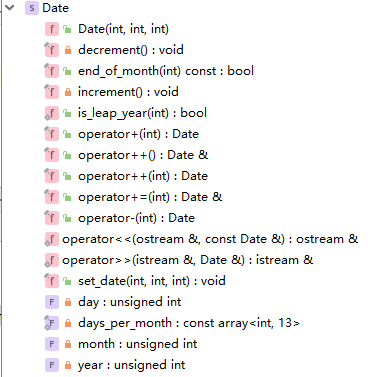
\includegraphics[scale = 1]{structure_date.png}
        % \includegraphics有两个参数,方括号中的可选参数设定了宽度
        % 可选参数有[scale=放缩因子][height=高度][width=宽度]
        % 第二个参数是文件名,放在源文件目录
        \caption{date 结构图}% 给插图加上编号和标题
        \label{fig:date}
      \end{figure}

  \subsection{Room 类}

    简单的room实现如图\ref{fig:room}

    % figure 环境,就是插图使用的浮动体环境,相当于普通段落,没有缩进
      \begin{figure}[H]% 可选参数ht表示可以出现在文字所在处(here)或顶部
        \centering% 后面内容居中
        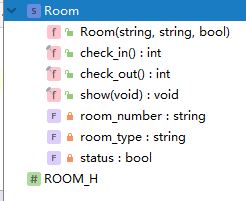
\includegraphics[scale = 1]{structure_room.png}
        % \includegraphics有两个参数,方括号中的可选参数设定了宽度
        % 可选参数有[scale=放缩因子][height=高度][width=宽度]
        % 第二个参数是文件名,放在源文件目录
        \caption{room 结构图}% 给插图加上编号和标题
        \label{fig:room}
      \end{figure}

  \subsection{Guest 类}
    简单的Guest 类如图\ref{fig:structure_guest}
    \begin{figure}[H]
        \centering
        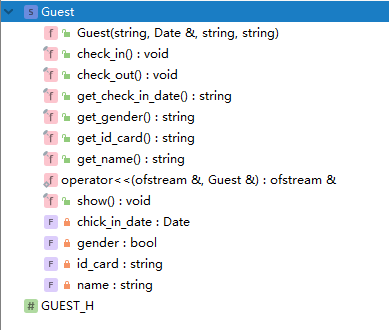
\includegraphics[scale = 1]{structure_guest}
        \caption{guest 结构图}
        \label{fig:structure_guest}
      \end{figure}

  \subsection{Csv 类}
    将对csv的操作封装成类,结果如图\ref{fig:structure_csv}
    \begin{figure}[H]
        \centering
        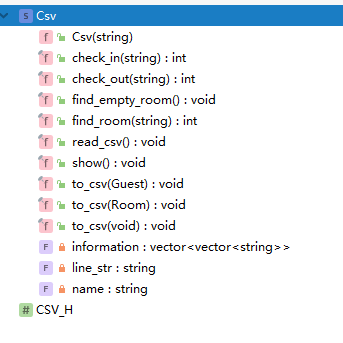
\includegraphics[scale = 1]{structure_csv}
        \caption{csv 结构图}
        \label{fig:structure_csv}
      \end{figure}

  \subsection{Manage 类}
    将对所有操作封装成类,结果如图\ref{fig:structure_manage}
    \begin{figure}[H]
        \centering
        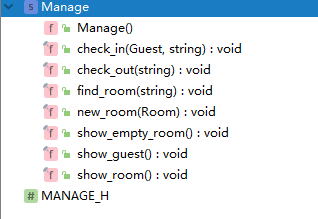
\includegraphics[scale = 1]{structure_manage}
        \caption{manage 结构图}
        \label{fig:structure_manage}
      \end{figure}
\section{调试分析}
  \subsection{guest 类的日期传递问题}
    在guest类中日期总是如图\ref{fig:bug_4},无法传递正确日期
    \begin{figure}[H]
      \centering
      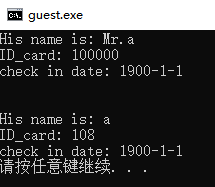
\includegraphics[scale = 1]{bug_4}
      \caption{所有日期都是1900-1-1}
      \label{fig:bug_4}
    \end{figure}
    经过测试(如图\ref{fig:bug_4_1}), date的复制构造函数没有问题
    \begin{figure}[H]
      \centering
      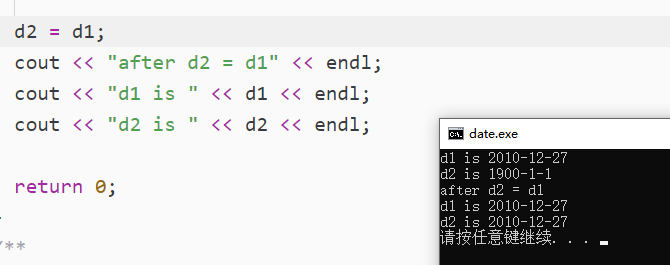
\includegraphics[width=0.8\textwidth]{bug_4_1}
      \caption{date的复制构造函数}
      \label{fig:bug_4_1}
    \end{figure}
    如图\ref{fig:bug_4_fix}最后在构造函数加了一个this指针解决,具体原因未知.
    \begin{figure}[H]
      \centering
      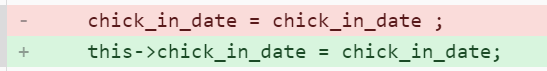
\includegraphics[scale = 1]{bug_4_fix}
      \caption{加了一个this指针解决}
      \label{fig:bug_4_fix}
    \end{figure}

  \subsection{csv 问题}
    使用csv文件格式时注意每个单元格不要带",",否则会视为两个数据单元

  \subsection{文件写入问题}
    测试中发现, 运行写入文件的代码之后展示表格的时候没有新增的记录信息(如图\ref{fig:bug_2})
    \begin{figure}[H]
      \centering
      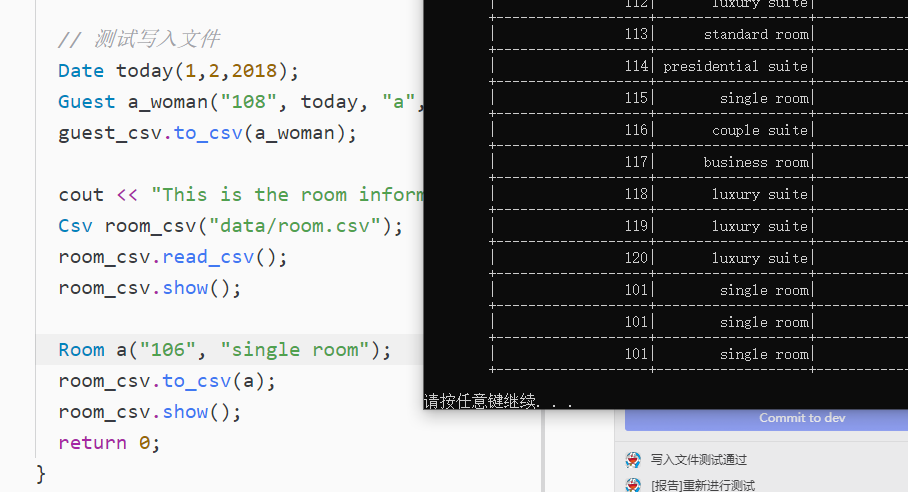
\includegraphics[width=0.8\textwidth]{bug_2}
      \caption{错误的录入}
      \label{fig:bug_2}
    \end{figure}
    原因:

    程序读取信息时调用函数"read\_csv()", 但是在调用函数"to\_csv()"写入文件时没有改变存储数据的数组"str\_array"


    解决方案:

    如图\ref{fig:bug_2_fixed},在"to\_csv()"函数体中调用一次"read\_csv()",即可重新载入数据,方便数据的再次查看
    \begin{figure}[H]
      \centering
      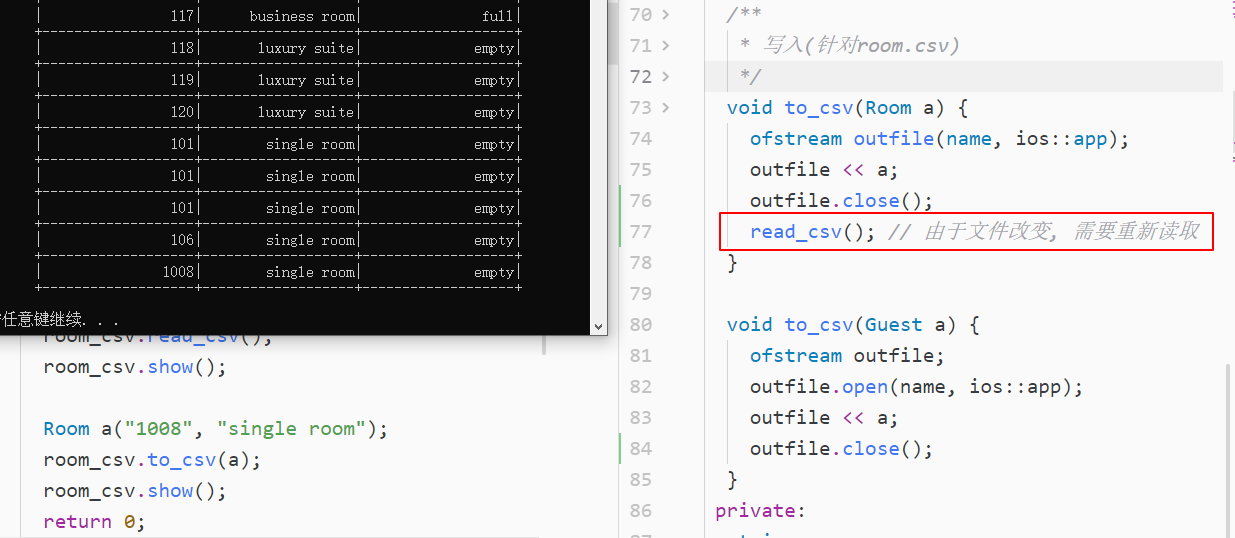
\includegraphics[width=0.8\textwidth]{bug_2_fixed}
      \caption{修复问题}
      \label{fig:bug_2_fixed}
    \end{figure}

    优化:

    在实际应用中,可能写入CSV之后不在使用,造成系统开销增大,可以设置标志(flag)在"show()"函数使用时检测是否调用过"to\_csv()",修改后测试结果如图\ref{fig:bug_2_more}

    \begin{figure}[H]
      \centering
      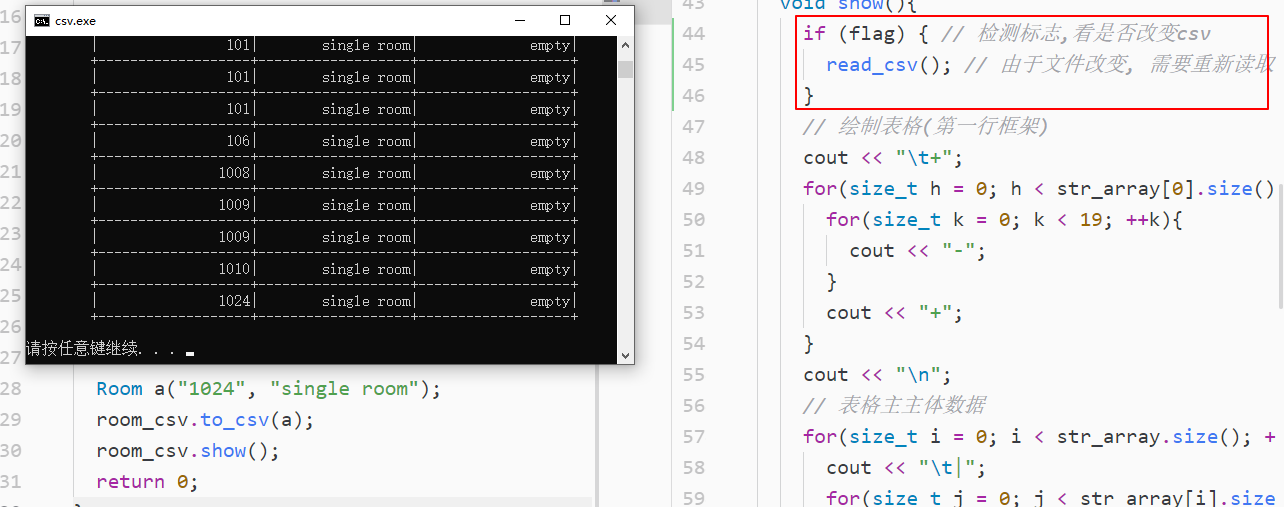
\includegraphics[width=0.8\textwidth]{bug_2_more}
      \caption{引入标志来减少开销}
      \label{fig:bug_2_more}
    \end{figure}

  \subsection{文件多次写入}
    经过以上调整优化, 发现每个表格打印了两次(如图\ref{fig:bug_3})
    \begin{figure}[H]
      \centering
      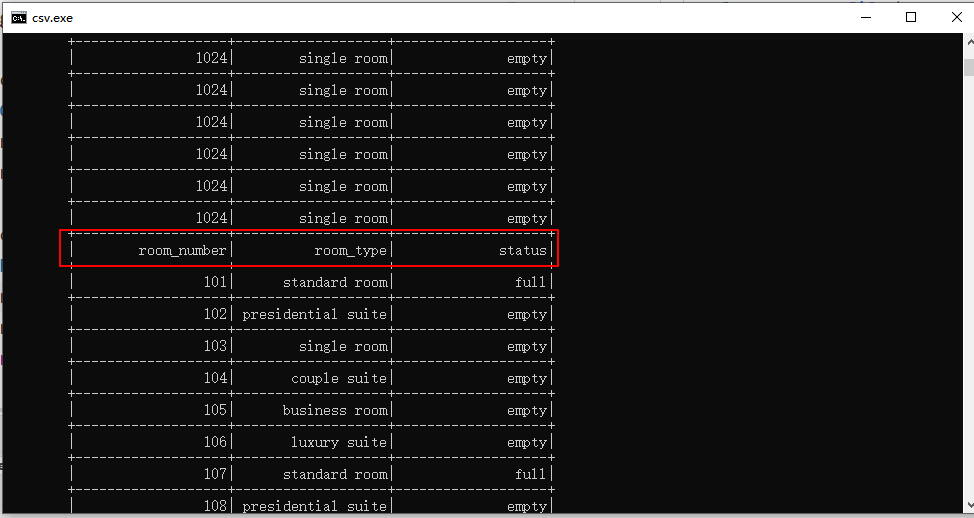
\includegraphics[width=0.8\textwidth]{bug_3}
      \caption{表格由于错误打印两次}
      \label{fig:bug_3}
    \end{figure}

    错误原因:

    由于"read\_csv()"是使用函数"push\_back()"入栈,重新调用相当于在原有二维数组的基础上增加内容,从而导致内容多次出现, 产生错误, 增加系统开销.


\section{用户使用说明}
  说明如何使用你编写的程序,详细列出每一步的操作步骤。
\section{测试结果}
  % 设计测试数据,或具体给出测试数据。要求测试数据完整和严格,能全面地
  % 测试所设
  % 计程序的功能。
  \subsection{单元测试}
    对于每个头文件, 对应一个测试.cpp文件,分别对date(图\ref{fig:test_date}),room(图\ref{fig:test_room}),guest(图\ref{fig:test_guest}),csv(图\ref{fig:test_csv}),manamge(图\ref{fig:test_manage})
    \begin{figure}[H]
      \centering
      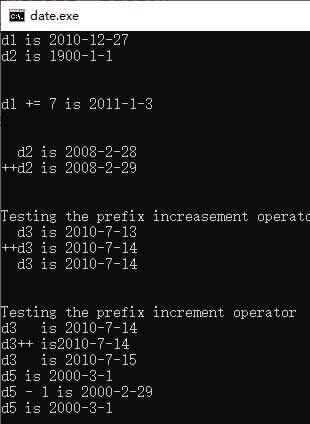
\includegraphics[scale=1]{test_date}
      \caption{date.cpp 对date类的测试}
      \label{fig:test_date}
    \end{figure}

  \begin{figure}[H]
    \centering
    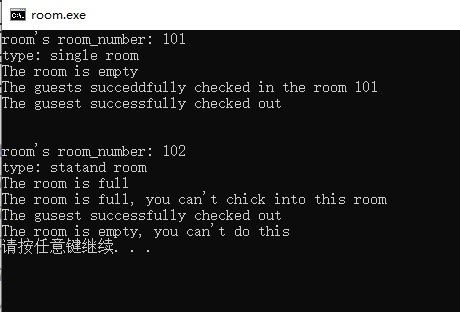
\includegraphics[scale=1]{test_room}
    \caption{room.cpp 对room的测试}
    \label{fig:test_room}
  \end{figure}

  \begin{figure}[H]
      \centering
      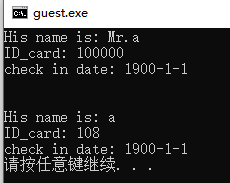
\includegraphics[scale=1]{test_guest}
      \caption{guest.cpp 对guest类的测试}
      \label{fig:test_guest}
    \end{figure}
  \begin{figure}[H]
      \centering
      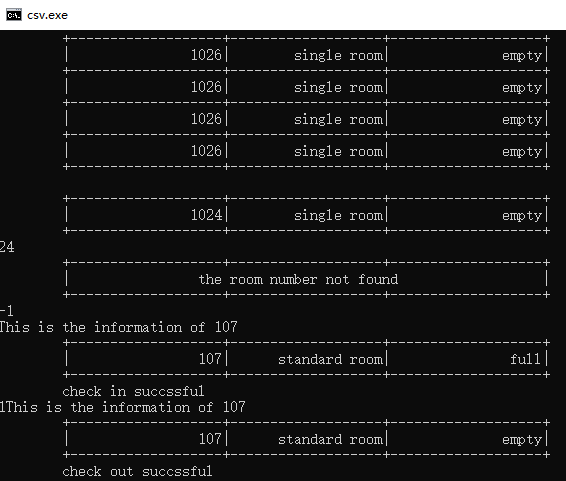
\includegraphics[scale=0.4]{test_csv}
      \caption{csv.cpp 对csv类的测试}
      \label{fig:test_csv}
    \end{figure}
  \begin{figure}[H]
      \centering
      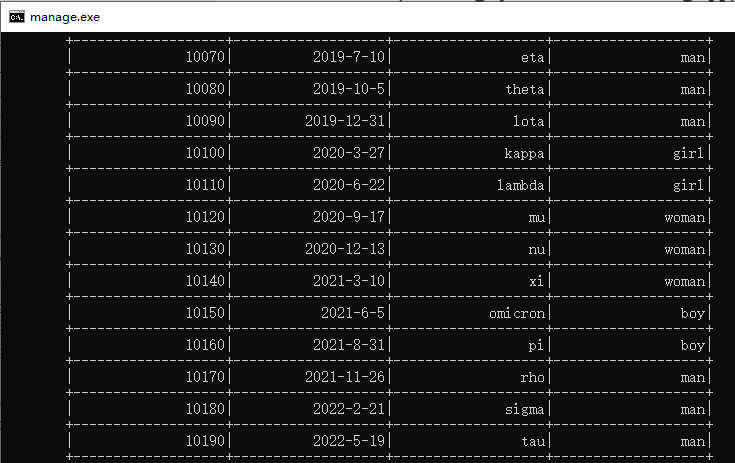
\includegraphics[scale=0.4]{test_manage}
      \caption{manage.cpp 对manage类的测试}
      \label{fig:test_manage}
    \end{figure}

\section{程序设计总结}
  在这次程序设计中, 探索各个模块的应用和项目的结构,开始习惯查阅参考文档$^{\cite{cpp_document}}$, 同时开始学习开源目录的代码规范$^{\cite{styleguide}}$, 写代码开始注重简洁.

  其中, 谷歌代码规范给我很多启发, 对于新手来说告诉我什么叫好看简洁的代码.$^{\cite{google_style}}$
  当然, 以为水平技术原因,只看懂了部分代码规范, 但是许多特性可以让开发更有条理

  在程序设计中, 我学会了用程序设计的思维考虑问题, 遇到了很多设计的问题, 看出对程序设计者学习能力的要求, 开发程序会不断遇到问题, 要通过互联网和文档资料学会解决, 探索更多的新技术,新方法,新理念.
  这一次尝试了git的分支功能, 知道了开发工具对效率的重要性.

  由于时间关系, 大多数功能不够完善, 代码不够简洁, 需要更多时间来完善重构, 新增功能时由于开始时考虑的疏忽, 功能函数归类错误, 导致代码冗长,混乱,还需要花时间维护.


\nocite{cpp_primier}% 只在参考文献中显示,不直接引用
\bibliography{reference} % 提示从reference数据库获取文献信息,来打印参考文献

\end{document}
